\documentclass{article}
\usepackage[utf8x]{inputenc}
\usepackage{latexsym}
\usepackage{amsmath}
\usepackage{float}
\usepackage{graphicx}
\usepackage{booktabs}
\usepackage{url}
\usepackage{subcaption}
\usepackage{hyperref}
\usepackage{booktabs}
\usepackage{adjustbox}
\usepackage{breakcites}

\title{Gender Bias in Language from a Natural Language Processing Perspective}
\author{Shawon Ashraf \\ st170090@stud.uni-stuttgart.de}
\date{29 September 2021}



\newcommand\BibTeX{B{\sc ib}\TeX}
%\addbibresource{bib.bib}

\begin{document}

\maketitle

\section*{Introduction}
Language is one of the most powerful and expressive mediums for humans to express their ideas. However it does not stop at being only a tool for communication, language also influences how humans perceive and build their thought process. This inadvertently dictates how humans develop a notion of structure and entities, for example society, class, gender etc. As Ludwig Wittgenstein had famously said that the limits of our languages define the limits of our cognitive boundary. Since language is a necessary prerequisite to describe any entity or class, which in this paper will be human gender, brings the question that if we can think of the social structure with our language and build around it, does the biases and stereotypes, specifically the ones towards gender get into language as well? Or is it that they are intertwined with human cognition and thus get carried over to the language we use for daily communication. Furthermore, for any Natural Language Processing task, language is the source of data, be it written (text corpora) or spoken (as speech signals). So this brings another question into light, if language can get biased from human cognition and the same language is used as a source for NLP applications, how much such biases affect NLP applications and our usage of language in our daily lives? In this paper, we look forward to finding answers for such queries and explore how gender bias is embedded in the ways we use our languages.

\section*{Gender in Language}
% How gender is perceived in language
To begin our discussion, we first need to look at how gender is defined in language in a formal way. As described in \cite{menegatti2017gender}, languages can be categorized \cite{braun2005cognitive} as Genderless Languages (Finnish, Turkish etc.), Natural Gender Languages (English etc.) and Grammatical Gender Languages (German, Italian etc.).

\noindent
\\
The key differentiator in this categorization is how gender is described in the lexical expressions of a language. Genderless languages do not have grammatical gender for nouns or pronouns, rather for words such as Mother, Father, Sister etc. they resort to what is described as "sex-marking". In Natural Gender Languages, pronouns are used to differentiate between genders and nouns can refer to both male and females, e.g. Doctor, Teacher, Nurse etc. Grammatical Gender Languages have their nouns distinguish between male and female entities and often, the female counterpart of a male word is inflicted from the male word. For example, in German, the female for \textit{Lehrer (Teacher)} is \textit{Lehrerin}. Again, the gender of a word is often defined by the surrounding parts of speech, e.g. \textit{Löffel(Spoon)} is masculine and \textit{Gabeln(Fork)} is feminine. To keep our discussion on point we are going to focus solely on the natural use of gender in language with sex-marking instead of grammatically motivated gender since it corresponds to the topic at hand.

\section*{Social View of Gender}
According to \cite{larson2017gender}, gender can be perceived as a social construct in the following ways : 


\begin{figure}[H]
    \centering
    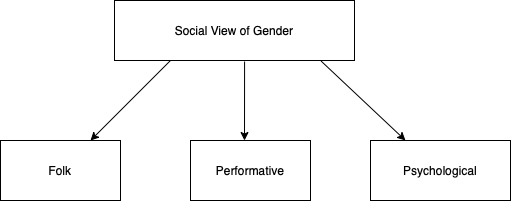
\includegraphics[width=0.8\textwidth]{Gender Social View.png}
    \caption{Gender as a social construct}
    \label{fig:gender_social_view}
\end{figure}

\noindent
The folk refers to common beliefs regarding gender orientation in a society. These views can be motivated by age old traditions or religion or both. The folk point of view regarding gender can be limiting depending on the culture and other factors and also a big contributor to our topic discussion which is bias towards a specific gender. We will discuss this effect in a later section of the paper. \\


\noindent
The performative view towards gender is based on what roles society assigns to a gender and expects people to conform to. These roles can be motivated by the folk point of view but the society can also have its own. For example in matriarchal societies in many Asian countries, women are regarded as the key figures and they have the final say when it comes to taking decisions. Likewise in a different form of society, the norms will expect that some tasks or occupation to be handles only by the male members while their female counterparts should maintain the households. We can also say that this a more constrained and imposed view of gender. \\

\noindent
The psychological view on the other hand is not constrained by society or traditional norms. This view rather focuses on the characteristics(such as self-reliance, independence, loyalty, sympathy etc.) of the existing gender and tries to find a cluster based on these characteristics. \\

\noindent
However, \cite{larson2017gender} also suggest that devising a hierarchy like the one described here is an open ended task and is much more dependent on the research question on what someone expects to do with gender. 

\section*{Gender Bias in Linguistic Processes}
We have seen how gender in language can be motivated by the linguistic structure as well as social structures in the previous sections. The question is, how do they connect to each other? From a neutral perspective, linguistic or grammatical role for words should not effect how they are imagined in a social hierarchy, however the reality is the opposite. \\

\subsection*{Gender stereotypes}
The first case of gender bias is traced in verbal communication and the roles of communicators in it \cite{menegatti2017gender}. Here, the problem is considered two fold, one being gender stereotypes, which expects gender specific traits or choice of words for communication, the second being considering male form as the general prototype of a human being in many languages. \\ 

\noindent
Gender stereotypes expect communal or softness or warmth based traits from females and agentic or more competitive traits from males \cite{cuddy2008warmth}. For example, a common gender stereotype would be to compare women with flowers while comparing men with wars and weapons. Such stereotypes lead to role related words being tied to a specific gender. In turn, this leads to giving male roles more power and status, as such roles of higher stature have mostly been held by men in history. This is the social effect, when we connect it to language, we can see that systematically marking some roles for a specific gender creates a cognitive conception that only the gender in contention is suitable for such roles and not the other, thus introducing gender discrimination in the process. This discrimination translates to language when these roles get described in language and over the time get integrated in the structure of the language.

\subsection*{Linguistic Conventions and Abstractions}
Linguistic conventions on the other hand tend to be gender neutral towards treating words. Despite that, existing gender stereotypes make gender bias normative and over time, the same linguistic conventions can no longer remain neutral. Again, linguistic abstraction becomes another way to introduce gender bias \cite{ng2007language}. There can be words with multiple meanings based on the context and when the users of a language tend to use such words in a specific context, they subconsciously bring forth their gender stereotypes \cite{rubini2014strategic}. \\ 

\noindent
This entire process becomes a cycle of social roles for genders transforming to gender stereotypes and then eventually making their way into daily use of a language. We can also assume here that gender bias is language has no single contributor, rather it is influenced systematically, as language, society, human cognition are all intertwined. 

\subsection*{Male as a general prototype in languages}
According to \cite{eagly1994people}, communal roles for women are more to assert male dominance in the society and attribute women more as a subordinate to men. This inadvertently creates a stereotype that men should be prioritised over women to describe a human prototype. This falls in line with ancient scriptures and texts depicting men as leaders, warriors and intellectuals mostly, while women in history fade into oblivion. \\ 

\noindent
Furthermore, this attitude influences the lexicon of a language as well. For example, words or entities such as \textit{Virgin}, \textit{Working Mother}, \textit{Career Women} etc. have no male counterparts \cite{budziszewska2014men} \cite{maass1996language}.

\subsubsection*{Masculine Generics}
To extend the topic of perceiving male as a general or generic prototype, we need to look at masculine generics and how they favor males over females. Generic forms for gender comprise mostly of masculine words whereas feminine words are only used to describe female entities. Frequent usage of masculine forms as generics validate the subconscious  gender stereotypes in language users. This can also be associated with the term \textbf{linguistic normativity effect} \cite{menegatti2017gender}, where people tend to associate general forms of a language to a gender which they think should be prioritized. As such, masculine generics, due to their nature of usage, do not consider men and women to be equal and due to women being less relevant to generics, they fail to contribute as a generic entity. Studies from \cite{braun2005cognitive}, \cite{sczesny2016can} have shown that when people are asked to assign a gender to some entity they do not know about, they tend to choose masculine gender more over feminine. When applied to a professional setting, e.g. \textit{Sports}, this stereotype can lead to the notion that in a specific occupation or field of work, women are always outnumbered by men \cite{stahlberg2007representation}. 


\section*{Gender Bias in NLP}
So far we have been discussing how gender bias plagues language and how it stems for various norms and stereotypes. Now we move on to various applications of natural language processing which are also affected by gender bias. 


\subsection*{Ghost in the shell or bias in data}
NLP applications such as, Machine Translation, Sentiment Analysis, Text Classification etc. use text corpora as their source. In a typical natural language processing setup, any text data or corpus is first represented in a numerical format, then passed as input to a learning algorithm or to create a model of the data, which afterwards is used for inferring the outputs for the desired tasks. The key thing to note here is the stage between input and the output, also known as the intermediate stage, where any machine learning or predictive algorithm will try to create an understanding of the data it has been fed (hence the term modelling). Depending on the algorithm at use, this intermediate process can either be very simple and explainable, such as Naive Bayes classifiers for finding spam emails to language models based around Transformer architecture such as BERT \cite{devlin-etal-2019-bert}, GPT \cite{brown2020language} etc. Let us put this intermediate step aside for a while and look at the input step. When we are converting text to numbers, e.g. bag of words, we are actually converting the contents of the text. So what is in the text becomes numeric inputs to NLP models. As a result, the gender bias in text gets numerically represented and when the models start learning this representation, they learn the bias in the text as well. This situation is similar to what we have discussed previously that bias gets systematically planted into language. In the following sections, we discuss some work done on evaluating gender bias in NLP applications.

\subsection*{Sentiment Analysis}
When we talk about sentiment analysis in NLP, we are generally referring to finding the emotion or sentiment conveyed in a piece of text. This can be as fine grained as inferring emotion labels such as joy, anger etc. to more generalized overviews, such as positive, negative, neutral. To discuss gender bias in sentiment analysis we are going to focus on \cite{kiritchenko2018examining}, where the authors try to evaluate if machine learning models exhibit human like bias and how it affects the overall results. \\


\subsubsection*{Affective bias towards gender}

\noindent
All the models evaluated in this study were submitted to SemEval-2018 for Task 1 "Affect in Tweets" where the goal was to find emotion and sentiment intensity in tweets. The authors hypothesized that when a model infers the emotion and sentiment inetnsity in a sentence, it should not be influenced by the gender or race of the subject in the person. For our discussion we are going to focus on the gender related analysis only.  \\

\noindent
To test their hypothesis against the submitted models, the authors created a benchmark corpus named "Equity Evaluation Coprus" or EEC in short. Their method checked if the output of a submitted system, which is the predicted emotion and sentiment intensity varies if the subject or person or entity in the input sentence has a different gender. If the output of their evaluation on the EEC deviated from their hypothesis, they kept note of which gender was assigned more of a specific set of emotions. Since NLP models learn the contents of the input, the authors made sure that their corpus was grammatically simple and short so that they analyze the outputs from the models. Their experiments on the submitted models showed that there was significant gender bias in the outputs of the models. The models assigned positive emotions to male entity names more than the female names. About 75\% to 86\% results showed gender bias. When analyzed, it was found that the models were prone to the same communal and agentic role oriented stereotypes we discussed earlier. For example, emotion labels such as joy, ecstatic etc. were more associated with male names and labels similar to fear, anxious etc. were associated on the opposite side.

\subsubsection*{Source of the bias}
Despite using a simple sentence structure corpus, the models exhibited gender bias. So the question arises, what is the source of this bias? Do models have subconscious bias like us humans? Models only learn distributions from numeric data, so if models get biased in the process it can entirely random and a different set of algorithms may exhibit different results. Another question can be asked that, most of the state of the art NLP models make extensive use of word embeddings such as Word2Vec \cite{mikolov2013efficient}. These embeddings are trained on text data from varied sources, which can contain gender bias. For example, if a word embedding was collected from newspaper text only, then it only has the representation of a more formal language, which can be prone to using masculine generics and other stereotypes. So the source of the word embedding can be worth exploring. The authors are of the opinion that there is no simple answer to where the bias actually comes from and consider it as a topic to be further explored and experimented on.

\subsection*{Biased Word Embeddings}
In the last section, we talked about gender biased word embeddings and how the source of the word embeddings can affect it. In their work, \cite{bolukbasi2016man} show that word embeddings can indeed get gender bias from the text they were trained with. For example, engineers are pre-dominantly male while women are more associated to house-wives. Word embeddings are essentially trained in an unsupervised approach, meaning, they only have the input data and no reference label to check their output against. So for example if someone trains word embeddings from San Tzus Art of War, the embeddings will only have knowledge on military and warefare. Since generalized word embeddings exhibit gender bias, a case can be made that the training data for the word embeddings be free from gender bias or have very minimum amount of it. (This falls into the area of debiasing which we shall discuss in a later section of this paper.). 

\subsubsection*{Contextualized word embeddings}
Word embeddings such as GloVe \cite{pennington2014glove} and Word2Vec have a singular representation for all the text in the corpus. They are not context sensitive. So even if there are multiple context sensitive usages of a word, it will still have a one single embedding for all the contexts. On the other hand, word embeddings from ELMo \cite{peters2018deep} are contextualized. Since contextualized embeddings learn the context of the word, they should be better able to infer the meaning of a word in a specific context and also learn the gender properly as well. While the first part of this assumption is true, the latter is not. \cite{zhao2019gender} have shown that ELMo shows significantly more gender bias in a Coreference Resolution task than a similar system based on GloVe \cite{lee2018higher}, in fact bias in the ELMo based system in their experiment showed 30\% more bias than the GloVe based system. Also, while analysing their results the authors made some interesting revelations. First, the training data for ELMo contained an imbalanced ratio of male to female entities, which they found to be 1$:$3. Second, the encoding process or the conversion process of ELMo does not give equal emphasis to both genders, hence resulting in a skewed distribution, biased more towards males.  \\

\noindent
Since word embeddings are unsupervised learners and going to learn the distribution in the training data, we can say here that input or training data is perhaps the biggest culprit in inducing gender bias. Coreference Resolution, as stated earlier, is one of the tasks where gender bias is almost omnipresent. In the next section, we are going to discuss about this. 


\subsection*{Coreference Resolution}
In coreference resolution, the task is to map multiple expressions to the same entity. For example, Simba said he would not go to the elephant graveyard. Here Simba and he are the same person. Hence the task is to map he to Simba. While this seems trivial on paper, we would like the reader to recall that when people are not sure which gender to assign to an entity they end up using the masculine gender. Coreference Resolution is not immune to this normative effect either. \\

\noindent
\cite{rudinger-etal-2018-gender} applied coreference resolution to infer how gender bias can affect a system which predicts occupation of an entity from text. Their evaluation showed that the gender bias in the outputs of the systems they tested were similar to real world gender bias statistics in the employment sector. Also, their results found that when the systems encounter ambiguity, especially with neutral gender words, they tend to randomly assign an occupation. They opine that the systems or models overgeneralize on gender specific terms. \\ 

\noindent
This again brings us back to the earlier sections of the paper where we said that the social roles of genders give more status quo to males over females. Since this mindset is inherent in language, the models trained on corpora collected from general sources will exhibit this problem as well. 

\subsection*{Machine Translation}
Gender bias in Machine Translation stems from coreference resolution, which we have discussed in the previous section. To describe this problem in a natural tone, let us take this example from \cite{saunders-byrne-2020-reducing} $:$ \textit{The doctor told the nurse that she had been busy.}. If a human had been asked to figure out who "she" here is, they can easily say that "she" is the doctor. However, this task is difficult for a coreference system \cite{gaut-etal-2020-towards} and even more critical in a machine translation setup. Outputs in machine translation are sequential, with each part relying on the previous one. This can be compared to a chain, where each component is tied to the previous one. As a result if one part gets a wrong translation, the error will propagate through the rest of the outputs as well. \\

\noindent
Let us reconsider the Folk view of gender again. In many cultures, either motivated by religious or traditional beliefs the concept of gender is binary and anything else is almost rejected. However, concepts such as gender are not rigid, and many languages at present have adopted more gender neutral wordings for pronouns and professions to keep up with social changes \cite{misersky2019grammatical}. This poses a big problem for languages which are yet to adopt a newer overview of gender. As a result when translating from languages with the newer overview to older ones, the output is more likely to suffer from qualitative issues. 



\section*{Mitigating Bias in Language}

\subsection*{Using Gender Fair Expressions}
In many cases, masculine generics can indeed be replaced with gender fair or gender neutral words. Especially in case of profession related words where studies from \cite{bem1973does} have shown that gender neutral wordings for position resulted in an increased interest from women to apply. However, gender fair expressions have also caused double sided effects \cite{horvath2016does}, where using word pairs have resulted in the opposite effect of creating more opportunities for men instead of creating equality. So this remains a topic for further exploration and careful curation, especially, we need to consider how to devise gender neutral wordings such that they do not create the aforementioned double-sided effect.

\subsection*{Conscious usage of language}
\cite{menegatti2017gender} call for a more consciuous and well aware usage of language, which involves understanding the present sex-marking and gender stereotypes in language and finding a way out of this situation. Although they consider gender fair expressions to be a solution, they also mention the issue discussed above and opine that this notion should be explored further. Moreover, there are more abstract notions of gender which do not get covered in gender opportunity related studies and often these abstract concepts are not made clear to the common mass, which should also be considered. For example, the call to legalize same sex marriage has met with hostility in many places, especially where people hold strong traditional beliefs, as such, paranoia and misinformation often create a wrong conception about this issue.  

\section*{Mitigating Bias in NLP}


\section*{Conclusion}
Sum up alles

\clearpage
\bibliography{bib.bib}
\bibliographystyle{acl_natbib}

\end{document}
